\documentclass{article} % This line defines the type of document. 'article' is a common class for small documents.
\usepackage[margin=1.3in]{geometry}
\usepackage{graphicx}
\usepackage{titlesec}
\usepackage{caption}
% \usepackage{hyperref}
\usepackage[colorlinks=true, linkcolor=blue, citecolor=blue, urlcolor=blue]{hyperref}
\usepackage{amsmath}

% \emergencystretch=3em

% Set paragraph indentation to zero
\setlength{\parindent}{0pt}

\titleformat{\section}
  {\normalfont\large\bfseries}{\thesection}{1em}{}

\begin{document} % This line marks the beginning of the document content.


\noindent\makebox[\linewidth]{\rule{\textwidth}{1pt}} 
\vspace*{0mm} % adds vertical space before the title
\begin{center}
    \Large\textbf{Toy Models of Superposition Replication and Findings}
\end{center}
\vspace*{2mm} % adds vertical space before the title
\noindent\makebox[\linewidth]{\rule{\textwidth}{1pt}}
\vspace*{0mm}

\begin{abstract}
\begin{quote}
    Toy Models of Superposition\cite{elhage2022toy} is a groundbreaking paper published by 
    researchers affilated with Anthropic and Harvard University in 2022. By 
    investigating small models with under 100 neurons, the paper demonstrates 
    that neural networks can represent more features than they have demensions. 
    Additionally, they use these so called ``toy models'' to understand the 
    relationship between how neural networks are trained and how they represent 
    the data internally. The original paper is quite extensive. As a result, this
    replication focuses on reproducing the most important results from the  
    introduction and sections 2 and 3 of the original paper. It also includes some
    comentary on section 1. This document may be expanded to include more 
    examples or other sections in the future.
\end{quote}
\end{abstract}
\section{Introduction}
The orginal paper motivates the idea of superposition with the following graphic:

\begin{figure}[h]
    \centering
    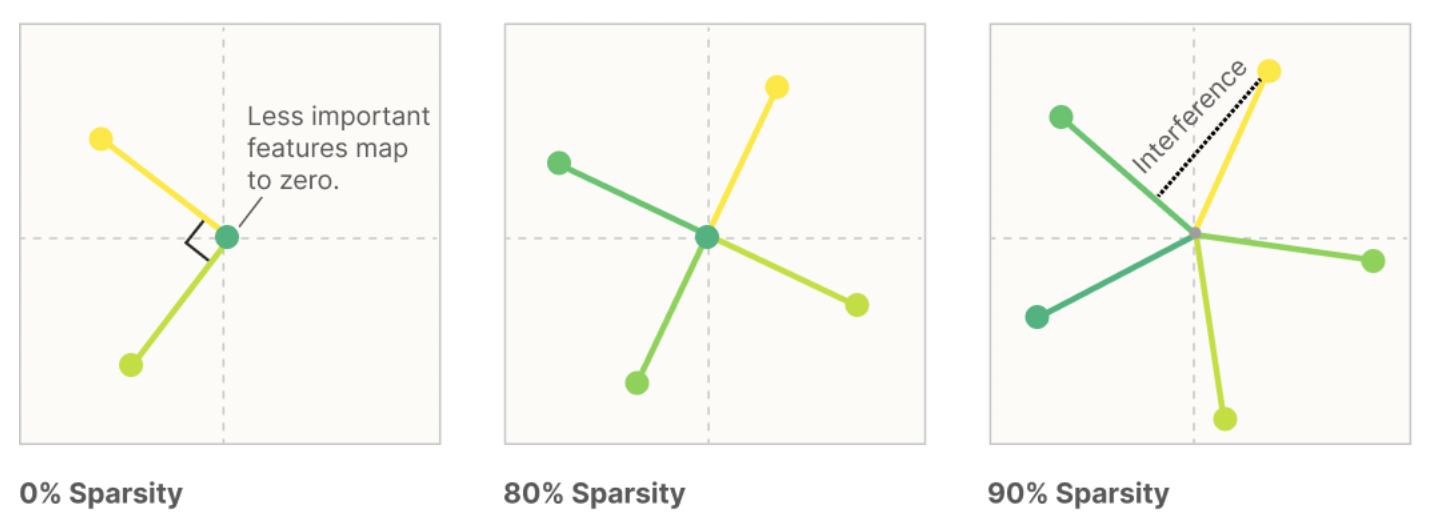
\includegraphics[width=0.55\linewidth]{section_1/images/section1_anthropic_graphic_.png}
    \captionsetup{font=footnotesize} % Set the font size for this caption
    % \caption{Graphic from Anthropic Paper}
    \label{fig:section1_anthropic}
\end{figure}

The basic idea is this: if you think of each feature as being represented inside of a
neural network by a direction, you can graph these directions and observe them.
By doing this, the authors of the original paper demonstrate that the way
a model maps features as directions depends on the sparsity of it's training data.
A replication of this phenomenon can be found below and the code used to 
generate it can be found 
\href{https://github.com/zroe1/toy_models_of_superposition/blob/main/section_1/section_1.ipynb}{here}.\\ 

\begin{figure}[h]
    \centering
    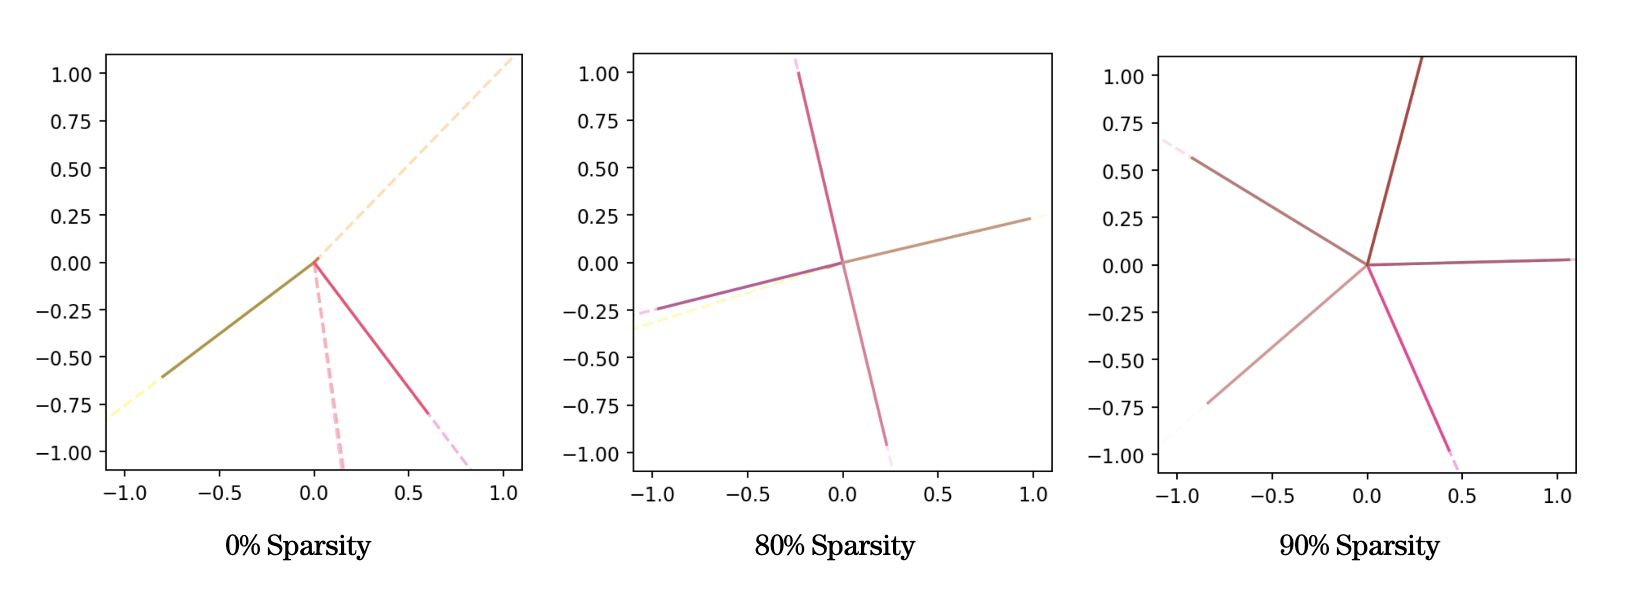
\includegraphics[width=0.6\linewidth]{section_1/images/section1_replicated_graphic.png}
    \captionsetup{font=footnotesize} % Set the font size for this caption
    \caption{Graphing superposition in 2D.}
    \label{fig:section1_replication}
\end{figure}

The model studied in  Figure~\ref{fig:section1_replication} is designed such that 
each column in the weight matrix corresponds to a  given input. Becasuse the weight
matrix only represents 2 neurons, the columns of the matrix can be graphed in
2D. As a result, it is trivial to plot the columns as 2D vectors (each representing 
individual features of the input). Obersving these vectors while increasing the 
sparsity of the model's input reveals
that the model can be trained to represent many more features than it has dimensions
(despite having only 2 neurons, the model in Figure~\ref{fig:section1_replication} 
can represent up to 5 features!). This is what the authors call "superposition." In 
future sections we will study superposition extensivly and produce the phenomenon
in larger networks.

\section{Background and Motivation}
In this section of Toy Models of Superposition\cite{elhage2022toy}, the authors
provide context and define terms.  In this paper, I make a few additional comments 
about some of the key ideas from this section. \newline \newline
\textbf{(1) Defining Features: }The original paper Toy Models of Superposition
defines features broadly as ``properties of the input which a sufficiently large 
neural network will reliably dedicate a neuron to representing.'' The authors do
however describe this definition as ``slightly circular'' and note that they are
not ``overly attached to it.'' I find the definition especially problematic because a network that is small or
has unconventional architecture may represent a feature that a larger network
or a network with a more typical architecture may represent. These 
representations are clearly still features, but are not treated as so under the
original definition.\newline\newline
As a result, I propose an alternative definition: features are aspects of the
input that a neural network represents accurately with a significantly higher probability than 
a randomly initialized network. In other words, features are parts of the input 
that a model determines to be important enough to represent internally.\newline\newline
\textbf{(2) Role of linear Representations in Neural Networks: }The original authors
of the paper study interpretability by trying to understand the linear representations
within neural networks. It is worth noting that this isn't the only way to approach
mechanistic interpretability research. Understanding the role of non-linearities 
at each level is likely also very important (and perhaps more neglected).\newline\newline
\textbf{(3) Defining Superposition: } The original paper has a compelling yet
simple definition for Superposition: ``Roughly, the idea of 
superposition is that neural networks `want to represent more features than they 
have neurons', so they exploit a property of high-dimensional spaces to 
simulate a model with many more neurons.'' This is the definition I will use
throughout this paper.

\section{Demonstrating Superposition}

In the introduction, the authors of the original paper proved that models with 
two neurons could exhibit superposition (this result was reproduced in Figure~\ref{fig:section3_anthropic}).
In this section, however, the authors demonstrate that superposition
is also observable in models with more than two neurons. \\

Specifically, they begin by exploring models with 20 inputs and 5 neurons, 
ultimately proving that these models exhibit superposition under certain 
conditions. The authors demonstrate this by graphing $W^TW$ for the weight 
matrix $W$ in each model (shown in Figure~\ref{fig:section3_anthropic}). 
They represent positive numbers in the matrix as red and negative ones as blue. They also graph the length 
of each feature by treating each column in $W$ as a vector. Features that are 
orthogonal to others in $W$ are labeled black while features that aren't are labeled yellow
(the exact details for how this is calculated is discussed in \ref{sec:calc_super}).\\

\begin{figure}[h]
    \centering
    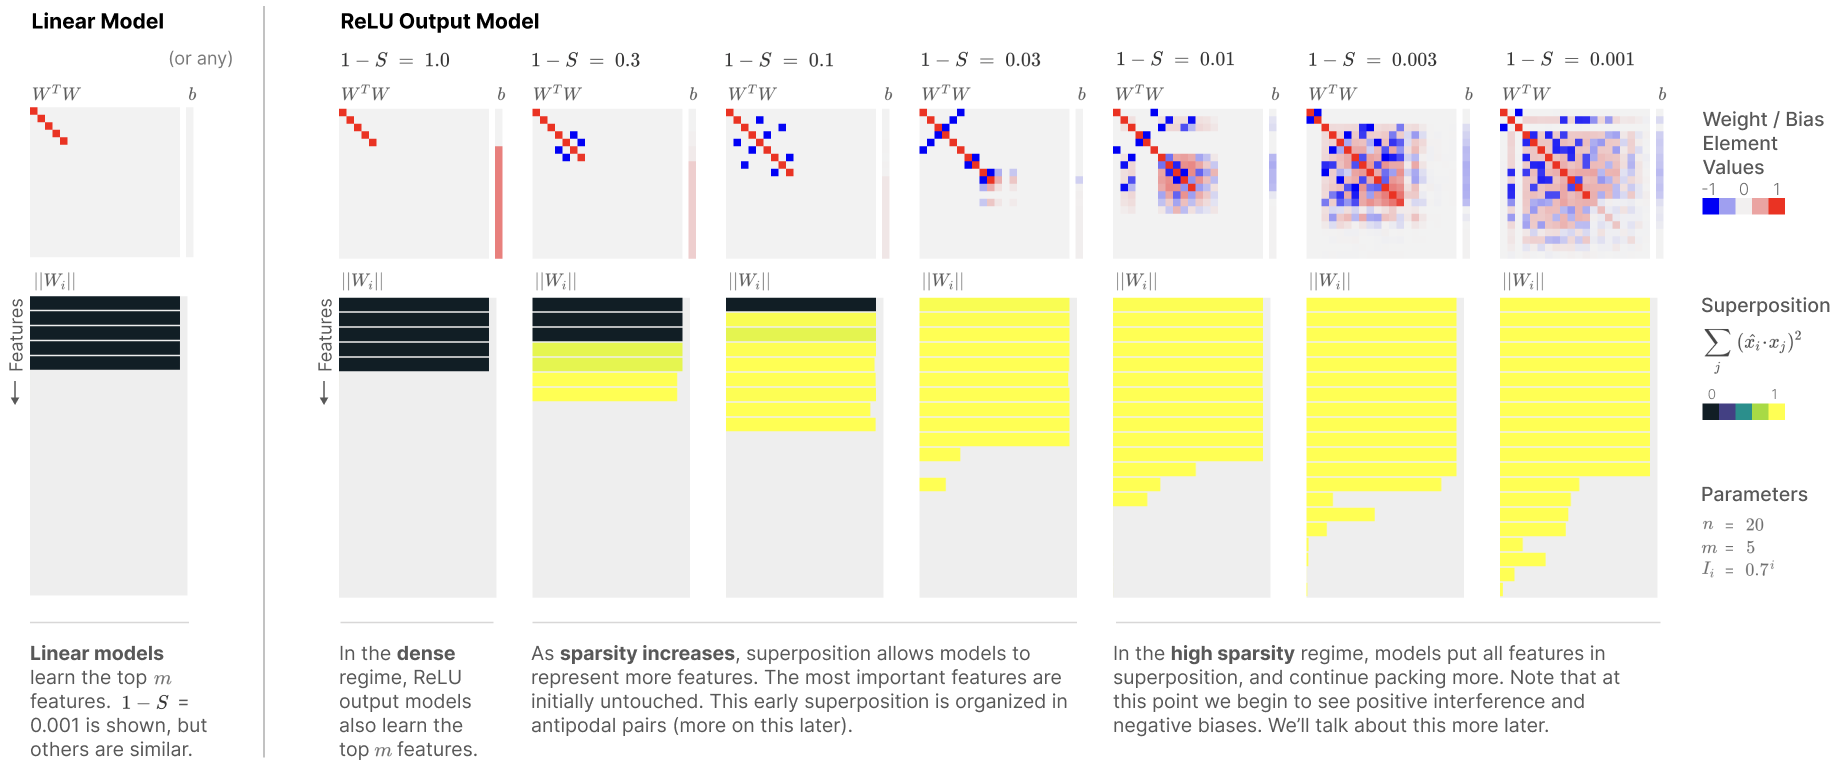
\includegraphics[width=0.9\linewidth]{demonstrating_superposition/images/anthropic_section3.png}
    \captionsetup{font=footnotesize} % Set the font size for this caption
    \caption{Graphs linear and ReLU models from Toy Models of Superposition \cite{elhage2022toy}}
    \label{fig:section3_anthropic}
\end{figure}

In Figure~\ref{fig:section3_anthropic}, the authors study both a linear model
and a model with a ReLU activation function. They found that both the linear
and ReLU model did not exhibit superposition in the absence of sparsity. By 
increasing the sparsity of the input, however, the ReLU model begins to clearly 
exhibit superposition by ceasing to represent features orthogonally.\\ 

The first step in replicating these findings was to train the linear and ReLU
models that don't perform computation in superposition. The linear model was
defined by $W^TWx + b$ and the ReLU model was defined by ReLU($W^TWx + b$). I trained both models
with Adam (learning rate = $1*10^{-3}$) on 20,000 batches of 256 examples.

\begin{figure}[h]
    \centering
    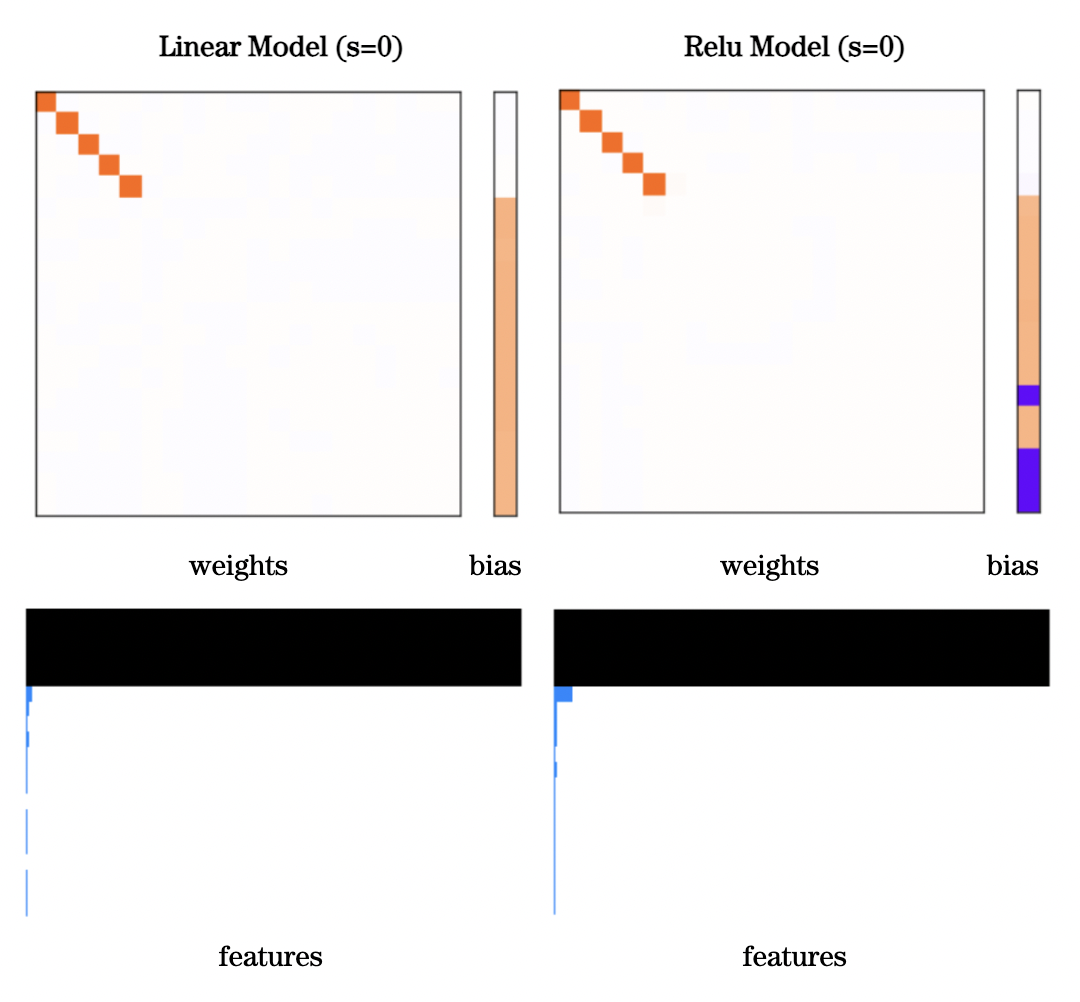
\includegraphics[width=0.4\linewidth]{demonstrating_superposition/images/relu_linear_0_sparsity.png}
    \captionsetup{font=footnotesize, width=0.7\linewidth} % Set the font size for this caption
    \caption{The generated graphics show that the model uses each of its five 
    dimensions to graph the 5 most important features orthogonally.}
    \label{fig:relu_linear_0}
\end{figure}

Note that in Figure~\ref{fig:relu_linear_0}, I use orange to indicate
positive numbers and purple to indicate negative ones. This is different from
the red and blue in Figure~\ref{fig:section3_anthropic}, to distinguish my work 
from that of the original authors. Similarly, while the original authors use 
yellow to indicate features in superposition, I use blue (This is hard to see in 
Figure~\ref{fig:relu_linear_0} but it will be more obvious going forward).

\subsection{Calculating Superposition}
\label{sec:calc_super}

The models in Figure~\ref{fig:relu_linear_0} do not exhibit superposition. They
encode each five most important features orthogonally (one feature for each
neuron in the model). Going forward however, we will be investigating models
that do not behave that way, instead encoding features as vectors that interfere
with eachother. In order to explain this phenomenon, and describe the graphs in 
Figure~\ref{fig:sparsity_1} it will be useful to dive a little bit into some
math. The color of the feature bars at the bottom of Figure~\ref{fig:sparsity_1}
are determined by the following equation.

\begin{equation}
\label{eq:my_equation}
\text{Interference} = \sum_{j \neq i} (\hat{W}_i \cdot \hat{W}_j)^2
\end{equation}

For a given column $i$ in weight matrix $W$, it calculates interference by taking
the dot product with every other column in $W$. Non-zero dot products indicate
that the columns in $W$ are not orthogonal. As a result, summing these dot 
products gives a general idea of how much the network is representing a given
feature in superposition. Note that $\hat{W}_i$ is the unit vector for $W_i$. 
This is necessary because when calculating interference, we are interested in
the direction of a given feature, not its length.\newline

In Figure~\ref{fig:sparsity_1} the length of a feature (calculated by taking the
length of the vector $W_i$) determines the lengths of the bars in the feature
graph. The interference equation (Equation~\ref{eq:my_equation}) determines the
color of the columns: black indicates a low value for Equation~\ref{eq:my_equation}
while blue indicates a higher value. Blue bars show that a given feature is represented
in superposition while black bars indicate that the feature is mapped orthogonally.
    

\begin{figure}[h]
    \centering
    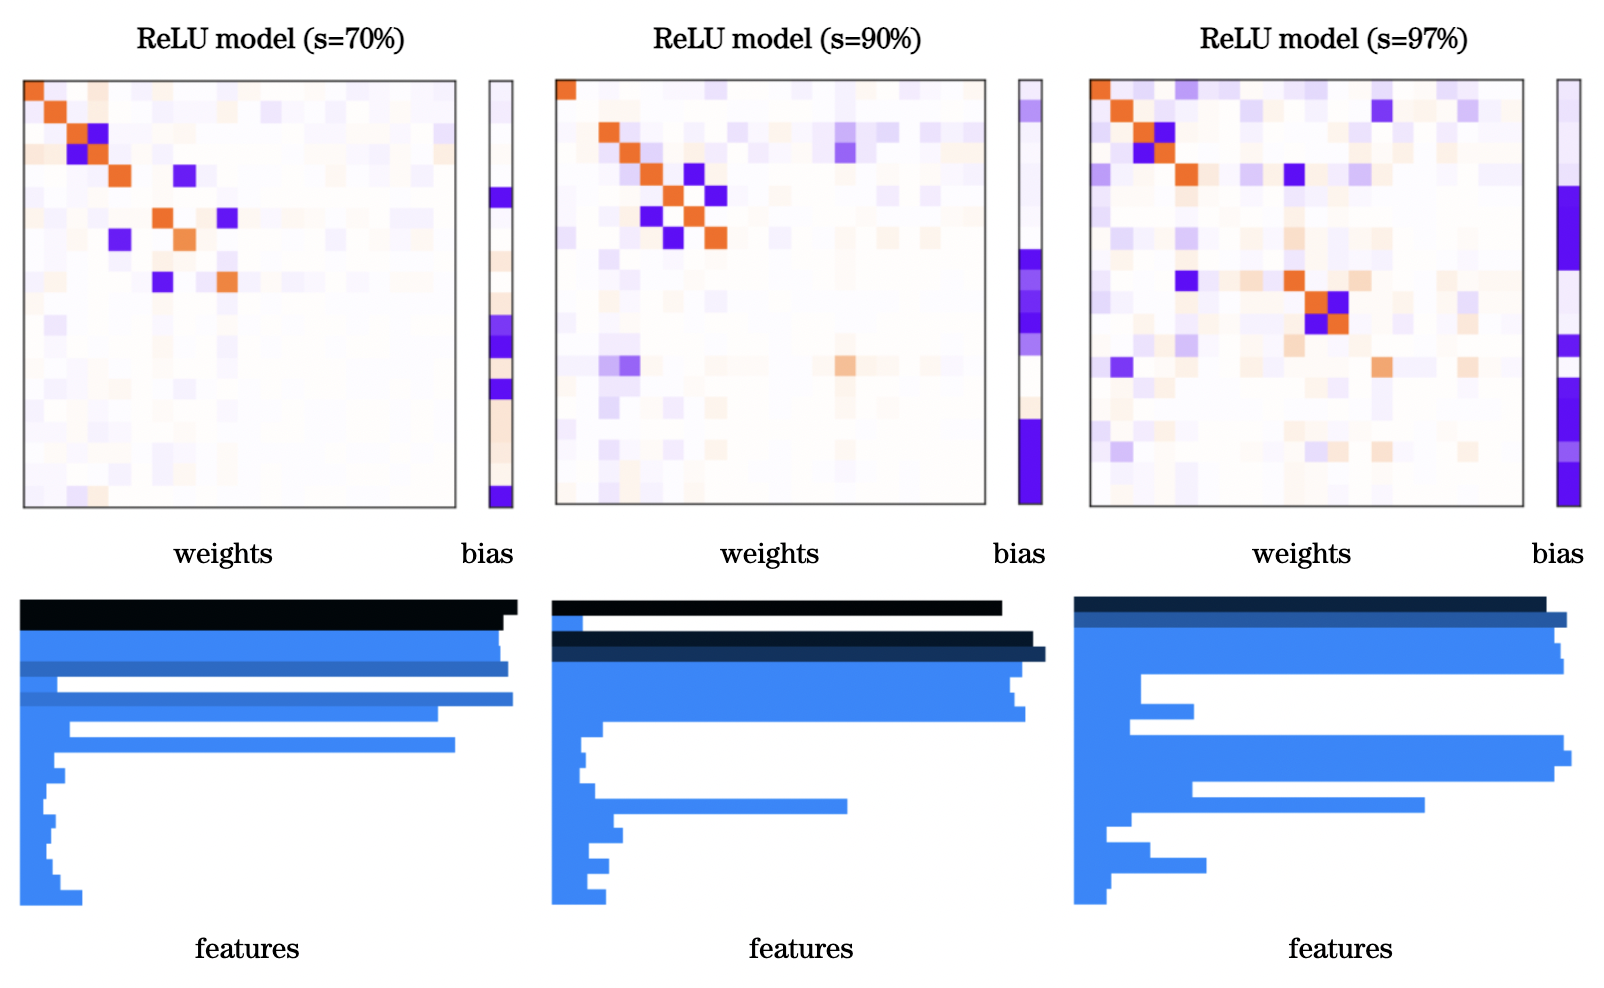
\includegraphics[width=0.75\linewidth]{demonstrating_superposition/images/sparsity_superposition1.png}
    \captionsetup{font=footnotesize, width=0.7\linewidth} % Set the font size for this caption
    \caption{
        By varying sparsity, superposition observed in ReLU models. This figure
        shows three models with increasing sparsity levels. As sparsity is increased, 
        more features are mapped in superposition.
    }
    \label{fig:sparsity_1}
\end{figure}


\begin{figure}[h]
    \centering
    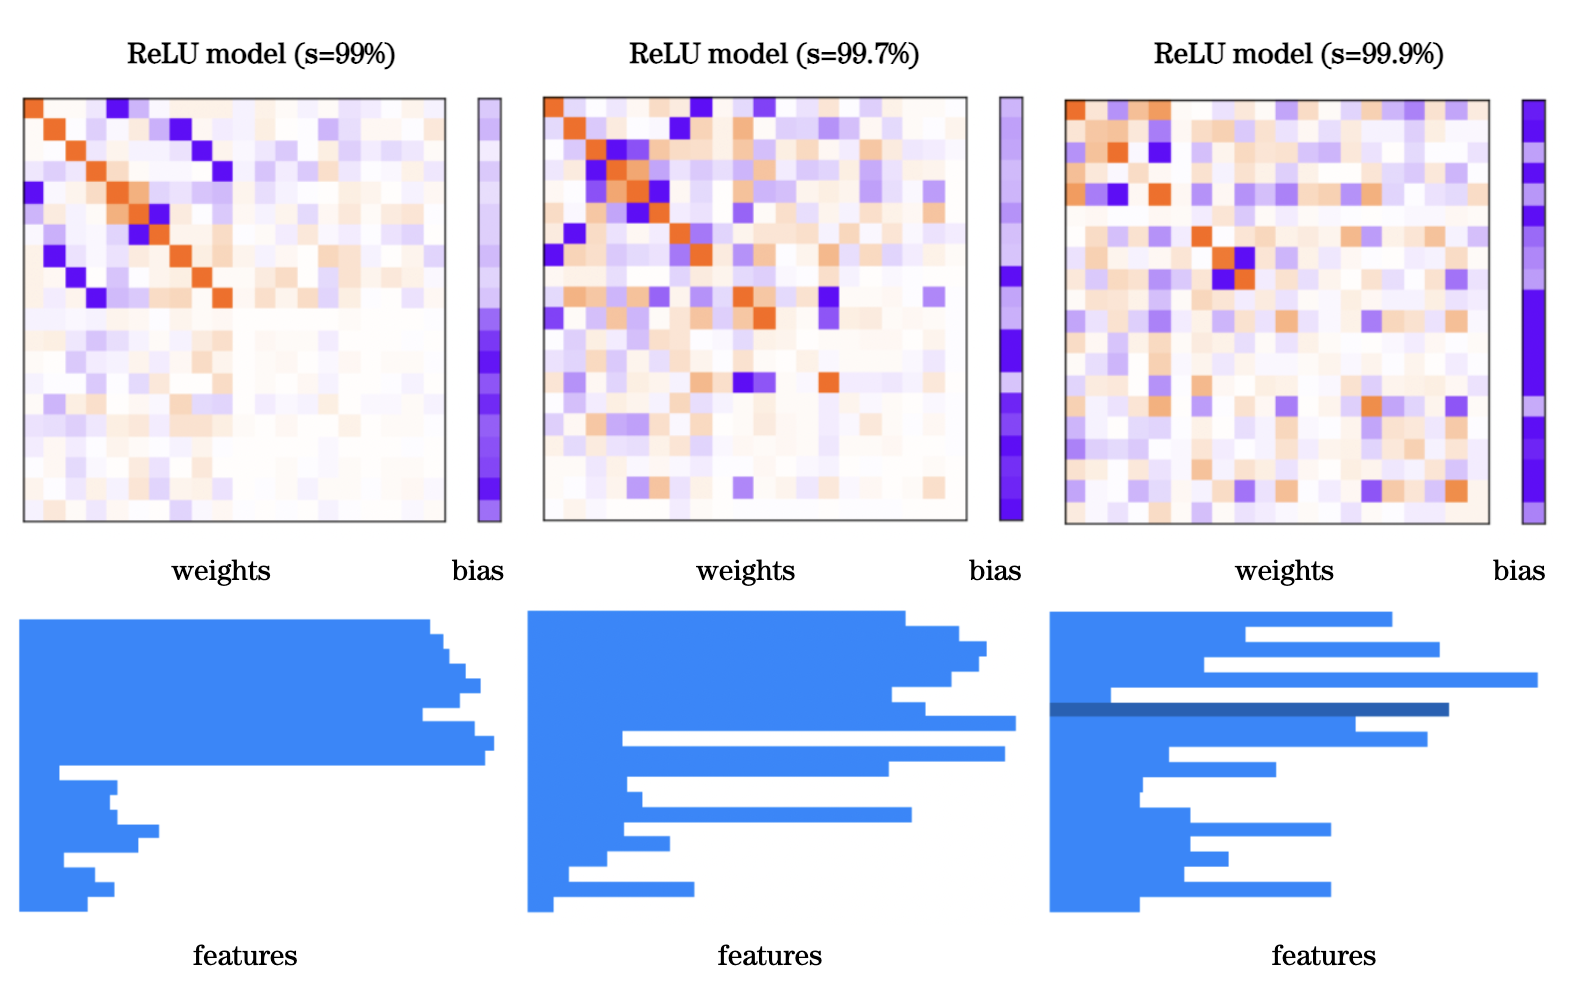
\includegraphics[width=0.75\linewidth]{demonstrating_superposition/images/sparsity_superposition2.png}
    \captionsetup{font=footnotesize, width=0.7\linewidth} % Set the font size for this caption
    \caption{
        By increasing sparsity even more, the model represents even more
        features in superposition.
    }
    \label{fig:sparsity_2}
\end{figure}

\bibliographystyle{plain}
\bibliography{references}

\end{document} % This line marks the end of the document content.
